% !TEX root = ../thesis.tex

\chapter{Návrh riešenia}
\label{methodology}

\section{Kontext využitia}

Nami vytvorený crawler bude zbierať dáta z vybraných slovenských spravodajských webov. Relevantné dáta uloží vo vhodnej forme pre následnú analýzu. Interagovať s ním bude iba jeden správca, schopný upravovať jeho kód. Riešenie teda nevyžaduje flexibilitu, zameriavame sa na jedno konkrétne použitie. 

\subsection{Analyzovanie zozbieraných dát}
Analýza dát nie je súčasťou a zameraním tejto práce. Jej popísanie, pre účely návrhu crawlera, považujeme za dôležité.

Dáta na analýzu budú konzumované ETL pipelinou postavenou nad Apache Sparkom (verzia 3.4.0) prípadne nad platformou Databricks (cloudová nadstavba Sparku). Očistené dáta budu analyzované Apache nástrojmi SparkML (Machine learning) a OpenNLP (natural language processing). Tie sú implementované v jazyku Scala a Java, bežiace na JVM (Java Virtual Machine).


Tieto frameworky podporujú jazyky Java, Scala, Python a R. Scalu považujeme za jasného favorita na budovanie robustných ETL procesov. A to hlavne vďaka jej plnej podpore a dobrej integrácii funkcionálnej paradigmy. Preto bude použitá v tejto časti a správca systému ho musí ovládať na dostatočnej úrovni.

Pre tento ETL proces uloženie dát v relačnej ani inej databáze neprináša žiadne benefity oproti uloženiu v jednom alebo viacerých klasických súboroch ako CSV, Parquet a podobne. 

Predpokladané zameranie analýzy bude sledovanie trendov, sentiment spoločnosti, klasifikácia do tém alebo identifikovanie najrelevantnejších článkov, napríklad pomocou backlink analýzy. 

V čase navrhovania crawlera, nám nie je detailne známe aké dáta si bude vyžadovať analýza. Považujeme to za miesto potencionálneho rozširovania funkcionality. 

\subsection{Nasadenie a zdroje}
Crawler by mal byť spúšťaný pravidelne, predpokladáme raz za mesiac. Prejsť by mal zopár slovenských spravodajských webov a zozbierať dáta na nasledujúce analyzovanie. 

Zdroje na infraštruktúru a údržbu sú veľmi malé. Predpokladáme, jedného správcu, s pár hodinami času do mesiaca. To musíme zohľadniť pri voľbe komplexnosti riešenia. 

Výpočtové a finančné zdroje sú taktiež minimalistické. Predpokladáme, že minimálne zber dát bude nasadený vo virtuálnom operačnom systéme bežiacom na fakultnom serveri. 



\section{Požiadavky}

\subsection{Paralelizmus}
Čakanie na odpoveď servera je hlavné výkonnostné obmedzenie. Preto požadujeme aby systém spracovával stránky paralelne. Týmto výrazne zvýšime efektívnosť a výkonnosť crawlera. 

\subsection{Odolnosť voči pádom} \label{sec:reqFailRecovery}
Predpokladáme, že systém bude bežať pár desiatok hodín. Nevieme zaručiť spoľahlivosť prostredia, v ktorom bude nasadený. Preto musíme rátať s možnými pádmi celého systému. 

Nechceme mrhať zdrojmi a časom, preto vyžadujeme aby systém bol schopný pokračovať v mieste kde skončil. Minimálne pokračovanie od posledného kontrolného bodu (checkpoint).

V ideálnom prípade by tento zotavovací mechanizmus mal byť nezávislí od prostredia. A zotaviť systém aj po preinštalovaní virtuálneho OS. Napríklad využitie služby DaaS (database as a service). Chápeme ale požiadavku na nízke náklady, ľahké nasadenie a jednoduchú údržbu. Preto sa uspokojíme aj s riešením v rámci jedného OS. Ale chceme aby riešenie bolo možné ľahko modifikovať na externý systém ukladania kontrolných bodov.

Za vhodné považujeme aj logovanie s nastaviteľnou úrovňou, pre zjednodušenie hľadania možných chýb.

\subsection{Obmedzená doména}
Zameriavame sa na extrahovanie dát z vybranej skupiny spravodajských webov. Túto skupinu chceme jednoducho upravovať, či už pridávať nové zdroje alebo redukovať existujúce. Táto časť riešenia by mala byť otvorená rozširovaniu. 

\subsection{Nízka komplexita, jednoduché nasadenie a údržba}
Potrebujeme aby systém bol ľahko udržateľný a nasaditeľný. Preto požadujeme aby systém bol čo najmenej komplexný. Znížená robustnosť a menej dostupných funkcionalít nám neprekáža. Potrebujeme najjednoduchšie riešenie čo zvládne vyriešiť náš problém, s čo najmenej zdrojmi (lightweight software). 

Očakávané úlohy údržby: \todo{formátovanie aby pekne sedelo}
\begin{itemize}
  \item Pridávanie a odoberanie cieľových domén.
  \item Oprava chýb.
  \item Úprava formátu a cieľa zozbieraných dát.
  \item Výber zbieraných dát.
  \item Spúšťanie nasadeného riešenia. 
\end{itemize}


\subsection{Požadované dáta na extrakciu}
\begin{itemize}
  \item Názov článku
  \item Úvodný paragraf, zhrňujúci článok.
  \item Hlavná časť článku.
  \item Mená autorov.
  \item Deň vydania. 
  \item Deň poslednej modifikácie.
\end{itemize}

Ako sme spomínali, očakávame úpravu požadovaných dát. Ako aj zbieranie doménovo unikátnych dát, teda dáta, ktoré nebudú musieť byť extrahované z celého korpusu prehľadávaných článkov (napr. komentáre článku). Neprekáža nám jednotný dátový formát, s neplatnými hodnotami v miestach nepodarenej extrakcie. 
Považujeme to za jedno z hlavných miest možného rozširovania systému, teda tieto zmeny musia byť robené rýchlo a jednoducho. 

\section{Vybrané technológie a prístup}
V tejto sekcii vyberieme technológie a jazyk, v ktorom vybydujeme náš crawler. Na základe toho navrhneme v ďalšej sekcii architektúru. 

Nie je našim cieľom vytvoriť distribuovaný, škálovateľný a vysoko výkonný crawlovací systém. Cieľom je jednoduché, nenáročné riešenie zamerané na úzky výber webových stránok. Bežiace raz za relatívne veľký časový úsek (plánujeme raz za mesiac). Teda nepôjde o kontinuálne crawlovanie, so zárukou čerstvosti dát. 

V požiadavkách je kladený dôraz na nízku komplexitu riešenia ako aj jednoduchosť nasadenia. Navrhujeme preto systém s čo najmenej funkcionalitami, splňujúci zadané potreby. Preto, ak sa to dá, chceme sa vyhnúť robustným frameworkom. 

\subsection{Výber jazyka}
Výsledný program bude bežať v tom istom prostredí ako program určený na analýzu zozbieraných dát. Z popisu kontextu nasadenia vyplýva prítomnosť JVM a nutná znalosť jazyka Scaly správcom. Pre úplnosť chceme zdôrazniť, že Scala sa kompiluje do Java byte kódu, spustiteľnom na JVM.

Využitím JVM a jazyka Scala aj v našom riešení sa vyhneme zvyšovaniu nárokov na správcu systému a na infraštruktúru. Ďalším benefitom je dizajn JVM, prispôsobeného na robustné aplikácie s dlhým až nepretržitým behom. Ako napríklad web server. 

Scala má vhodnú úroveň abstrakcie pre naše potreby, vysokú expresívnosť a plne podporuje funkcionálnu paradigmu. Tá vyniká v aplikáciach s vysokou paralelizáciou a dôrazom na dáta. Čo je aj naše použitie. 

Pre tieto dôvody ju vyberáme ako jazyk, s ktorým vybudujeme náš crawler. Kedže považujeme za benefitné použiť ten istý jazyk pre obe časti celkového riešenia, potrebuje v našom riešení použiť rovnakú verziu ako použije analytická časť. Použitá verzia Sparku - 3.4.0, podporuje JVM verziu 8/11/17 a Scalu 2.12/2.13. Nevidíme, žiadne podstatné rozdieli medzi týmito dvoma podporovanými verziami. Použijeme 2.12. \todo{zdroj na dokumentaciu https://spark.apache.org/docs/latest/}

\subsection{Výber technológie}


Pre Scalu existuje zopár knižníc na tvorbu crawlera. Sú postavené na mohutnom frameworku Akka alebo na funkcionálnych streamoch. 

Akka je dizajnovaná pre vysoko efektívny a distribuovaný systém. Nevieme si obhájiť jej použitie za cenu zvýšených nárokom na nasadenie a údržbu. 

Funkcionálne streamy sú vybodované nad knižnicou Cats. Ide o knižnicu poskytujúcu abstrakcie z teórie kategórii. Vyžaduje pokročilú znalosť funkcionálneho programovania. 

Zvolenie týchto riešení neprinesie pridanú hodnotu, vyrovnavajúcu výrazne zvýšenie nárokov na schopnosti správcu a komplexitu riešenia. Preto ich nepoužijeme. Myslíme si, že centralizovaný, teda nedistribuovaný crawler vybudovaný bežnými knižnicami a abstrakciami Scaly, bude dostačovať nášmu použitiu. Práve túto hypotézu si chceme overiť touto prácou.  

\subsection{Výber spôsobu ukladania extrahovaných dát} \label{subsec:pickSaving}
Pre navrhnutie architektúry je potrebné si stanoviť ako a kde chceme ukladať extrahované dáta. 

Prvá, typická možnosť na zváženie je \textbf{relačná databáza}. Očakávame pravidelné zmeny schémy ukladaných dát a chceme aby proces s tým spojený bol čo najmenej pracný. Relačné databázy typicky vyžadujú manuálnu úpravu schémy. Ich výhoda je záruka ACID vlastností a flexibilné dotazovanie. Pri dodržaní normálnych foriem dosiahneme deduplikovania hodnôt ako autor, dátum vydania, doména a pod. 

\textbf{NoSql} databázy riešia problém s pracným menením schémy ale vyžadujú prispôsobenie schémy predpokladaným dotazom. Keďže nepoznáme potreby analýzy, nevieme ani aké dotazy by boli požadované. 

Tretia možnosť je ukladanie do \textbf{CSV} alebo do efektívnejších formátov ako napríklad \textbf{Parquet}. Oproti predchádzajúcim možnostiam je zložitosť infraštruktúry výrazne nižšia, čo je jedna z hlavných požiadaviek. 

Crawler nebude dáta čítať, bude ich iba zapisovať. ETL proces, spracuvavajúci dáta na analýzu sa spustí až po jeho dobehnutí. Teda nemusíme sa obávať problémov so súbežným prístupom k dátam. Preto sú ACID vlastnosti nepotrebné.

Aktuálne požiadavky na systém budú rovnako splnené aj bez použitia databázového systému, teda ukladaním jednoduchých súborov priamo na súborový systém. Vyberáme si teda toto, menej komplexné a plne dostačujúce riešenie. 



\section{Návrh architektúry}

Pri návrhu staviame na základný algoritmus crawlovania popísaný v časti: \ref{sub:zakladnyAlgoritmusCrawlovania}\todo{Opravit cross referenciu}. Pridáva hlavne paralelizáciu a schopnosť vrátiť sa do stavu pred pádom programu. Hlavné moduly crawlera sú  extraktor, orchestrátor, repozitár a URL manažér (ďalej ako UM).  Na obrázku \ref{o:classDiagramVisitResult} sú znázornené pomocné triedy.

\begin{figure}[!ht]
    \centering
    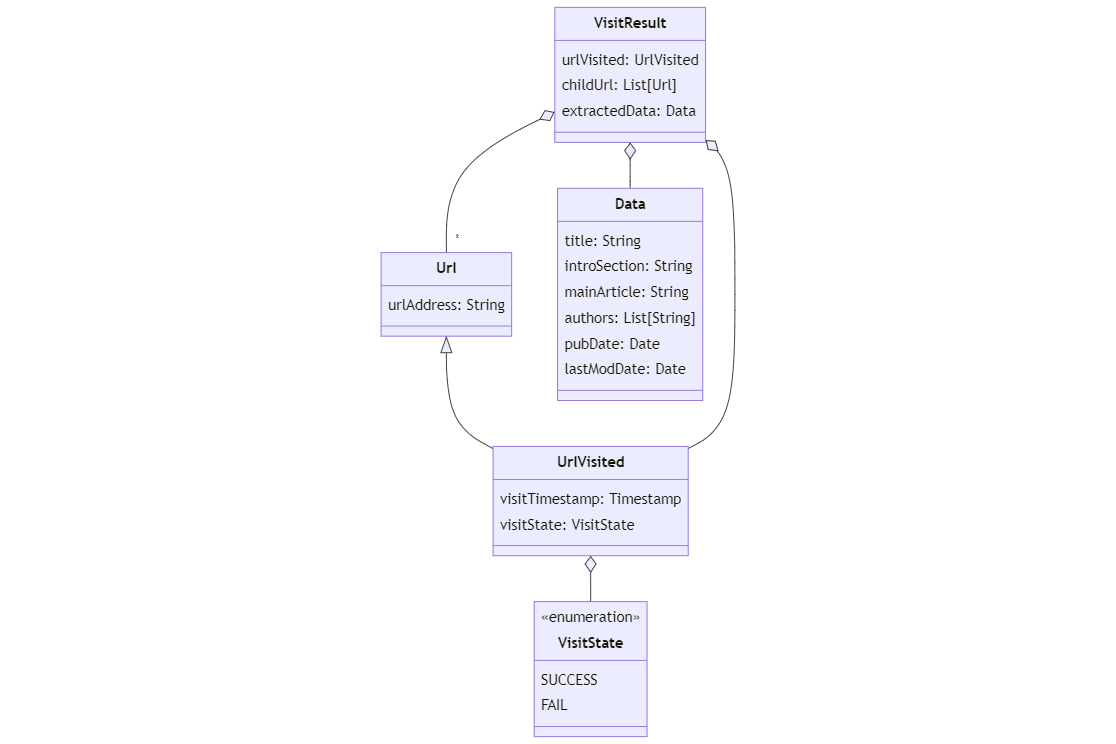
\includegraphics[width=.9\textwidth]{figures/classDiagramVisitResult.png}
    \caption{Class diagram pomocných dátových štruktúr \label{o:classDiagramVisitResult}}
\end{figure}

\todo{diagram vsetkych implementacii a interfacov}

\subsection{Orchestrátor}
Tento modul je zodpovedný  za paralelizáciu a integrovanie ďalších modulov. Stránky prechádza po krokoch, tie môžeme v zmysle požiadaviek nazvať checkpointy. Od UM dostane časť práce na jeden krok, teda kolekciu URL adries. Túto časť rozdelí pracujúcim vetvám (threads) na časti (chunky) a čaká kým dokončia svoju prácu. 

Následne agreguje výsledky navštívenia stránok. Do repozitára zapíše extrahované dáta. Druhú čast výsledku, URL nachádzajúce sa na navštívených stránkach, zapíše do UM. Nakoniec zapíše do UM v tomto kroku navštívené adresy. Týmto sa končí krok behu crawlera.

Keďže najprv zapisujeme do repozitára a až potom do fronty zodpovednej za obnovu stavu výpočtu po páde programu, sme nútení zopakovať maximálne jeden krok. Čím splníme požiadavku v sekcii \ref{sec:reqFailRecovery}. Môže nastať duplicitný zápis do repozitára v kroku, v ktorom padol program. To musíme zvážiť pri navrhovaní a implementovaní repozitára. 

\begin{figure}[!ht]
    \centering
    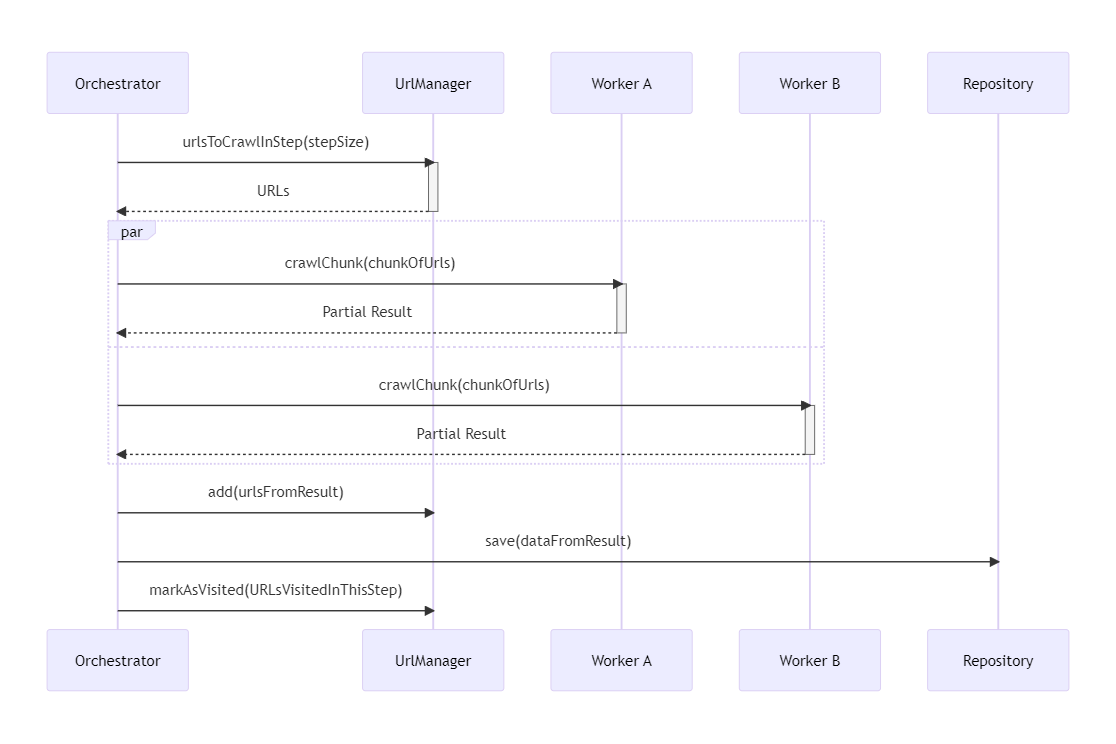
\includegraphics[width=.9\textwidth]{figures/seqDiagCrawlStep.png}
    \caption{ Sekvenčný diagram znázorňujúci jeden krok \label{o:seqDiagCrawlStep}}
\end{figure}



\subsection{URL Manažér}
Jeho zodpovednosť je poskytnúť URL adresy na navštívenie a to bez opakovania. Taktiež byť odolný voči pádom a reštartom ako je požadované v ref{sec:reqFailRecovery}.

Jeho obsah môže byť väčší ako operačná pamäť a v spojení s požiadavkou \ref{sec:reqFailRecovery} musíme jeho stav ukladať v externom úložisku. Môže ísť o malú súborovú databázu alebo obyčajný súbor. Pre potreby testovania a rýchleho vývoja navrhujeme implementovať aj UM nezávislé na externom úložisku. To ale bude podrobne riešiť v implementačnej časti. 


\todo{Navrhnutie aký externý systém použijeme}


\subsection{Repozitár}
Tento modul je zodpovedný za uloženie extrahovaných dát pre následnú analýzu. 

Z troch porovnaných možností v časti \ref{subsec:pickSaving} sme vybrali ukladanie do obyčajného súboru. Máme možnosti CSV alebo Parquet. 

Perquet je stĺpcovo orientovaný, s optimalizáciou prázdnych hodnôt. To umožňuje rýchlejšie čítanie konkrétnych stĺpcov. ETL proces konzumujúci naše dáta bude čítať celý súbor. Preto nám použitie tohto súboru neprináša osoh. Naopak jeho použitím zvýšime komplexitu riešenia. Preto budeme ukladať do CSV súborov priamo na súborový systém. 

Ako sme spomínali, prijali sme riziko dvojitého zápisu jedného kroku po reštarte systému. ETL proces bude pripravovať na analýzu, transformáciami, čistením a deduplikovaním. Nemáme veľký dôvod to teda riešiť aj v našom riešení. Musíme ale podotknúť nutnosť vynechať pri deduplikovaní stĺpec - Čas navštívenia, inak záznamy vzniknuté extrahovaním tej istej stránky v rozdielnom čase budú označené za chybné. 

Keby sme zapisovali do jedného súboru riskujeme prekročenie limitu veľkosti systému.

Každý krok preto zapíšeme do samostatného súboru, ako názov môžeme použiť napríklad časovú značku. Veľkosť súboru bude kontrolovaná veľkosťou kroku, teda počtom v ňom spracovaných adries. ETL proces bude spracovávať iba nové súbory. To dosiahne logovaním názvov spracovaných súborov alebo ich mazaním. 

\subsection{Extraktor}
Extraktor je zodpovedný za extrakciu releventných dát z navštívenej stránky ako aj extrahovanie URL adries. Extrahuje iba cieľové adresy, teda v ňom prebieha filtrovanie aké domény chceme navštíviť\todo{tu sa hodi aby sme v analyze zaviedli pojem focused crawler a cielove domeny alebo nieco podobne}. 

Podpora extrakcie stránky je prevedená implementáciou tohto interfacu. Napríklad extrakcia sme.sk bude prevedená v SmeExtraktor.

\todo{dopisanie sposoby filtorovania adreies a ako priraduje adrese extraktor + diagram}

\subsection{Prístup k paralelizácii}
Môže sa naskytnúť otázka, prečo si pracujúce vlákna nepýtajú adresy priamo od UM a svoju prácu nezapisujú do repozitára, ale robia to prostredníctvom orchestrátora? V nasledujúcich odstavoch si vysvetlíme prečo sme sa tak rozhodli a aké princípy nás k tomu viedli. 

Hľadanie chýb je v paralelných systémoch notoricky náročnejšie. Časť problému riešia základné princípy funkcionálneho programovania a to nemenné dátové štruktúry (immutables) a uprednostňovanie čistých funkcií (pure functions). 

Používanie nemenných štruktúr nám umožní zdieľanie zdrojov medzi vláknami bez potreby synchronizácie a uzamykania. To eliminuje riziko race condition\todo{prelozit}.

Čisté funkcie si vieme zjednodušene a nie úplne korektne definovať ako funkcie bez vedľajších efektov. Vedľajšími efektmi sú napríklad zápis alebo čítanie z databázy. Pre túto prácu je uvedená definícia postačujúca, nakoľko sa nezameriava na funkcionálne programovanie. \todo{Definovať lepsie mozno ked bude malo textu}. To znamená, že nepotrebujeme synchronizačné a zamykacie mechanizmy. Výrazný pridaným benefitom je jednoduché chápanie a predvídateľnosť. 

Program bez vedľajších efektov ale nerobí nič užitočné, keďže nevie interagovať s prostredím. Našou snahou teda nie je úplná eliminácia ale zníženie ich počtu a ich presunutie na hranice systému. Teda snažíme sa aby jadro systému bolo zostavené z čistých funkcii a vedľajšie efekty prebiehali iba na perifériách systému, s obmedzenou komunikáciou s jadrom. Nazveme to princípom separácie.

Scalu sme si vybrali aj kvôli plnej integracii funkcionálneho programovania, čo sa iných zvažovaných jazykoch povedať nedá. Preto tieto princípy uplatníme v najväčšej možnej miere. 

V popise URL Manažéra sme navrhli jeho perzistovanie. Čo si ale vyžaduje vedľajšie efekty. Uplatníme princíp separácie presunieme ho na perifériu programu a obmedzíme jeho komunikáciu so zvyškom programu. Komunikuje s ním iba orchestrátor.  Rovnaké dôvody platia aj pre repozitár. 

Aplikovaním týchto princípov sme zvýšili čitateľnosť programu a zlepšili testovateľnoť.  

\subsection{Kontext Crawlera}
Pre uľahčenie testovania sme separovali vedľajšie efekty do jednej triedy, nazvanej Kontext. Obaľuje repozitár, UM, loggovanie, a funkciu navštívenia stránky. Táto trieda je inicializačný parameter crawlera. Ide vlastne o injektovanie závislostí. 

Pri jej inštancovaní vieme použiť rôzne implementácie spomínaných modulov a tým modifikovať správanie crawlera. Takto vieme vytvoriť prostredie pre deterministické testy. 

Hlavne funkcia navštívenia stránky nám dáva plnú kontrolu nad crowlovaním pri testovaní. Parametrom je Url a výstupnou hodnotou je HTML Document. Pre každý test môžeme použiť špecifickú definíciu. Príklad takejto jednoduchej funkcie je zapísaný v pseudo kóde nižšie.

\begin{lstlisting}
//Pseudo code
input: Url to be visited: u
output: HTML Document

if u == "https://www.sme.sk/" :
    return SomeTestDocument
else 
    return invalid value


\end{lstlisting}


Pre testovacie účely sa môže použiť aj neperzistovaný repozitár a UM. Ide o podobnú techniku ako mockovanie\todo{PRELOZIT???} ale dosiahnutú bez reflexie. 

\begin{figure}[!ht]
    \centering
    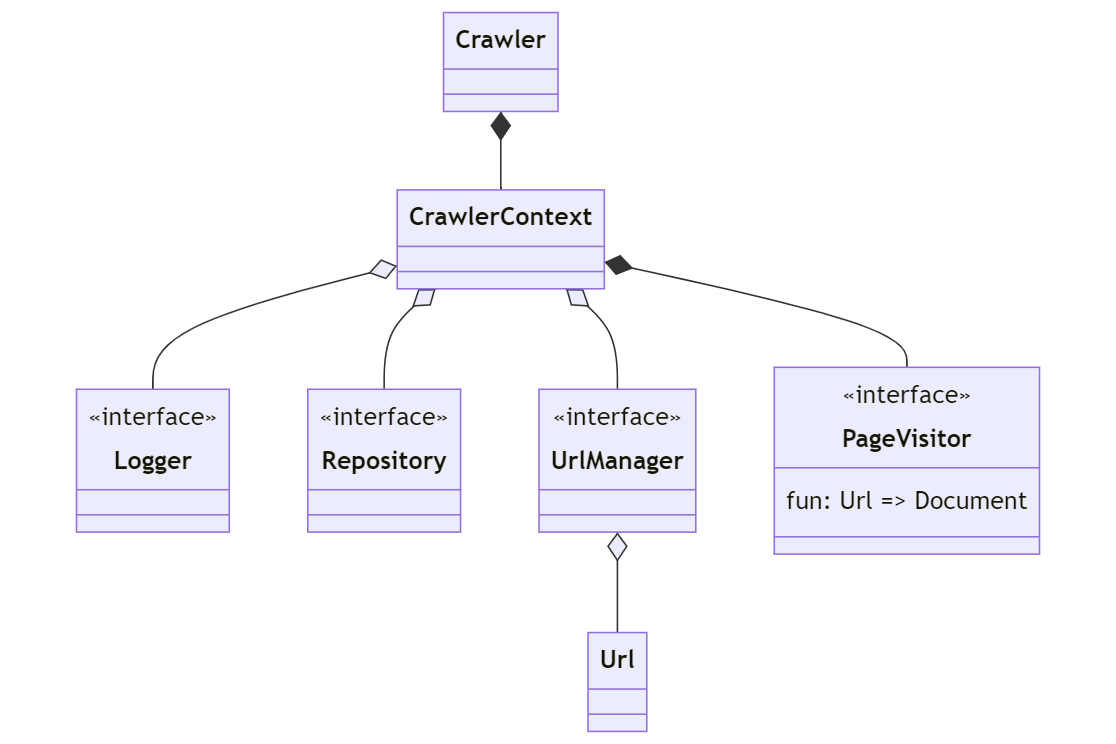
\includegraphics[width=.9\textwidth]{figures/classDiagramContext.png}
    \caption{ Class diagram Kontextu crawlera \label{o:classDiagramContext}}
\end{figure}